\documentclass{article}[12pt]
\usepackage[a4paper, margin=1in]{geometry}

% packages
%   formatting
%\usepackage[utf8]{inputenc}
\usepackage{url}
\usepackage{hyperref}
\hypersetup{
    colorlinks=true,
    linkcolor=blue,
    filecolor=magenta,      
    urlcolor=blue}
\usepackage{xcolor}
%\usepackage[T1]{fontenc}
%\usepackage{lmodern}
\usepackage{float}
%   math
\usepackage{amsmath}
\usepackage{amssymb}
%\usepackage{bbm}

%\usepackage{mathptmx}
%\usepackage{verbatim}
%\usepackage{bm}
%   figures, tables, ...
\usepackage{algpseudocode}
\usepackage{algorithm}
\usepackage{graphicx}
\usepackage{booktabs}
\usepackage{makecell}
%\usepackage{multirow}%http://ctan.org/pkg/multirow

% python
\usepackage{listings}
\definecolor{darkgreen}{rgb}{0,0.6,0}
\lstdefinestyle{Python}{
    showstringspaces=false,
    language        = Python,
    basicstyle      = \small\ttfamily,
    morekeywords = {as},
    keywordstyle    = \color{blue},
    stringstyle     = \color{darkgreen},
    commentstyle    = \color{darkgreen}\ttfamily,
	breaklines = true,
	postbreak=\text{$\hookrightarrow$\space},
	% style >>> and ... 
	%   see: https://tex.stackexchange.com/questions/326655/make-a-keyword-in-listings-enviorment
	alsoletter = {>,.} ,
    morekeywords = [2]{>>>,...},
    keywordstyle = [2]\color{cyan}\bfseries}

% bibliograpy
\usepackage{biblatex}
\addbibresource{ags.bib}
\addbibresource{main.bib}

% macros
\input ags.tex
\newcommand{\bvarepsabs}{\boldsymbol{\varepsilon}_\text{abs}}
\newcommand{\bvarepsrel}{\boldsymbol{\varepsilon}_\text{rel}}
\newcommand{\varepsabs}{\varepsilon_\text{abs}}
\newcommand{\varepsrel}{\varepsilon_\text{rel}}

\newcommand{\AGSComment}[1]{{\color{cyan} Aleksei: #1}}
\newcommand{\JRComment}[1]{{\color{violet} Jag: #1}}
\newcommand{\FJH}[1]{{\color{purple}#1}}
\newcommand{\scnote}[1]{ {\textcolor{blue}  {\mbox{SC: } #1}}}
\DeclareMathOperator{\Order}{{\mathcal O}}

% metadata
\title{Monte Carlo for Vector Functions of Integrals}
\author{Aleksei Sorokin, Jagadeeswaran Rathinavel}
\date{\today}


\begin{document}

\maketitle

\begin{abstract}
Monte Carlo methods present an efficient approach for approximating the expected value of a random variable. Algorithms exist to adaptively sample the random variable until a user defined error tolerance is satisfied with theoretical guarantees or with high probability. This work describes an extension of such methods which supports adaptive sampling to satisfy error criteria for vector functions of multiple expectations. Although several functions involving multiple expectations are being evaluated, only one random sequence is required, albeit sometimes of larger dimension than the underlying randomness. These enhanced Monte Carlo and Quasi-Monte Carlo algorithms are implemented in the QMCPy Python package with support for vectorized, economical function evaluation. We exemplify these capabilities on problems from machine learning and global sensitivity analysis.
\end{abstract}

\tableofcontents

\newpage

\section{Introduction}

Many quantities of interest may be formulated as functions of multiple expectations. In the simplest case one may be interested in computing a vector of expectations. Here the function combining expectations is the identity. A more nuanced case is approximating the ratio of expectations when computing the Bayesian posterior mean. More complex combinations of integrands are necessitated in other domains such as global sensitivity analysis where a quantity of interest is the ratio of one expectation to the difference of two other expectations.

Monte Carlo (MC) methods have proven to be an efficient technique for approximating a single expectation. Quasi-Monte Carlo (QMC) methods  offers even greater efficiency when the random variable we are taking the expectation of has low effective dimension. Numerous MC and QMC methods have been developed to adaptively sample the random variable and provide bounds on the true expectation that hold with high probability or even probability 1. Examples of such methods are discussed in Section \ref{sec:MCM}. 

This work extends a number of existing MC and QMC methods from \cite{tong2022guaranteed} to adaptively approximate a function of multiple expectations to within a user-specified error tolerance. Our extension incorporates shared samples, custom error bound propagation, multidimensional vectorization, and parallel function evaluation. The resulting routines are implemented into the QMCPy Python package \cite{QMCPy} which is distributed on both GitHub and PyPI. 

\section{Monte Carlo Methods} \label{sec:MCM}

Monte Carlo methods are well-suited to approximate the expected value a random variable. Suppose we would like to approximate the vector mean $\bmu = \bbE[\bf(\bX)] \in \bbR^{d_{\bmu}}$ where $\bX\sim\calU(0,1)^{d_\bX}$ and  $\bf: [0,1]^{d_{\bX}} \to \bbR^{d_{\bmu}}$ is a vectorized integrand. Monte Carlo methods compute 
\begin{equation*}
    \label{eq:mcapprox}
    \hat{\bmu} = \frac{1}{n}\sum_{i=1}^n \bf(\bx_i) \approx \int_{[0,1]^{d_{\bX}}}\bf(\bx)\D\bx = \bbE[\bf(\bX)] = \bmu
\end{equation*}
using $\bx_1,\dots,\bx_n \in [0,1]^{d_\bX}$ where the discrete distribution of $\{\bx_1\}_{i=1}^n$ is a good approximation of the true distribution $\calU(0,1)^{d_{\bX}}$. While the standard uniform choice for $\bX$ may seem restrictive, a variety of random variables are compatible in this framework after an appropriate variable transformation. For example, if we are interested in computing $\mu = \bbE[g(\bT)]$ for some $g: \bbR^{d_{\bX}} \to \bbR$ where $\bT \sim \calN(\boldsymbol{m},\boldsymbol{\Sigma})$, then $\mu = \bbE[f(\bX)]$ where $f(\bX)=g(\boldsymbol{A}\Phi^{-1}(\bX)+\boldsymbol{m})$, $\boldsymbol{\Sigma}=\boldsymbol{A}\boldsymbol{A}^T$, and $\Phi^{-1}$ is the inverse CDF of a standard normal distribution acting element wise. More details on variable transformations can be found in \cite{QMCSoftware} along with examples in the QMCPy framework.

\emph{Crude Monte Carlo} (CMC) methods choose sampling nodes to be independent and identically distributed (IID). That is, $\bx_1,\dots,\bx_n \simiid \calU[0,1]^{d_\bX}$.
The elementwise error in approximating $\bmu$ by $\hat{\bmu}$ using IID nodes is  $\calO(n^{-1/2})$. 

Quasi-Monte Carlo (QMC) methods choose sampling nodes in a carefully coordinated, dependent manner to avoid the gaps and clusters observed in IID nodes, see Figure \ref{fig:ld_seqs}. Discrepancy measures quantify how close the discrete distribution of such points is to the standard uniform distribution. The discrete distribution of QMC nodes have low discrepancy (LD) with the standard uniform distribution compared to IID nodes. Popular LD node sets include Halton points, digital nets, and integration lattices. It follows from the Koksma-Hlawka inequality, or similar quadrature error bounds, that the elementwise error in approximating $\bmu$ by $\hat{\bmu}$ with LD nodes is  $\calO(n^{-1+\delta})$ for any $\delta > 0$ \cite{dick2013high,hickernell1998generalized}. This convergence rate for QMC methods is significantly faster than the rate for crude Monte Carlo when $\bf(\bX)$ has low effective dimension. 

\begin{figure}[H]
    \centering
    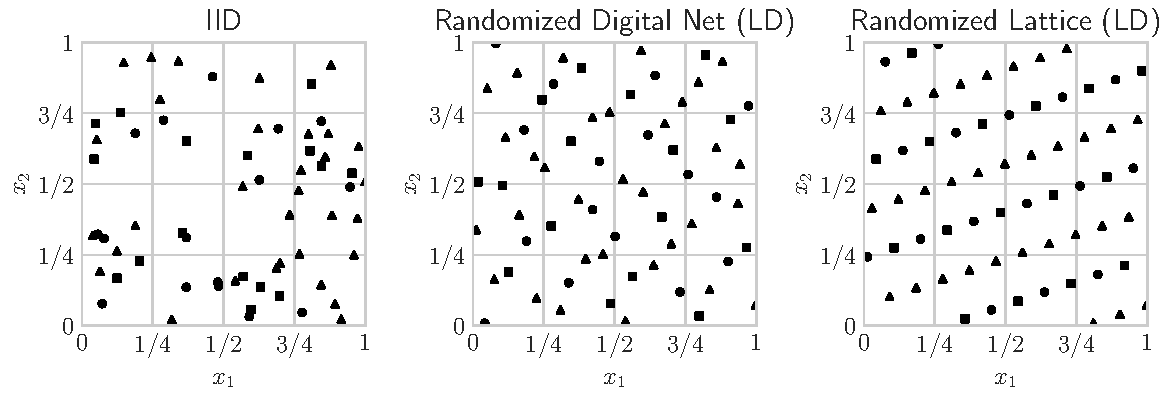
\includegraphics[width=\textwidth]{figs/ld_seqs.pdf}
    \caption{Contrast of IID and LD sequences. The first $2^6$ points of each sequence are shown in \AGSNote{cyan} with the next $2^6$ points in \AGSNote{magenta} and the $2^7$ points following that in \AGSNote{green}. Notice the gaps and clusters in the IID sequence contrasted with the more uniform coverage of LD sequences. Also notice that as the sample size is doubled the LD sequences fills in the gaps left by previous nodes.}
    \label{fig:ld_seqs}
\end{figure}

The QMC methods in this article rely on LD sequences that are extensible in both dimension and number of samples, again see Figure \ref{fig:ld_seqs}. This enables our algorithms to utilize shared point sets and adaptively increase the number of points used to estimate $\hat{\bmu}$ without needing to discard previous observations. Many LD sequences are implemented in base $2$ for computational efficiently and therefore prefer sampling the first $2^m$ nodes in the sequence to satisfy uniformity properties. Thus, existing QMC algorithms will iteratively double the sample size until the error bounds on $\bmu$ are sufficiently tight. As an example of generating a LD sequence, Algorithm \ref{algo:Gen.Lattice} details generating $R$ independent randomizations of a size $n=2^m$ lattice sequence. 

\begin{algorithm}[h!]
    \caption{$\texttt{Gen.Lattice}(R,n)$}
    \label{algo:Gen.Lattice}
    \begin{algorithmic}
    \Require $R \in \bbN$, the number of independent randomizations.
    \Require $n = 2^m \in \bbN$, the number of nodes in the lattice sequence.
    \\ \hrulefill
    \State fix $\bv \in \bbN^{d_{\bX}}$, a carefully chosen Lattice generating vector, see \cite{cools2006constructing,hickernell2000extensible} for details. 
    \State draw $\boldsymbol{\Delta}_1,\dots,\boldsymbol{\Delta}_R \simiid \calU(0,1)^{d_{\bX}}$
    \For{$i \gets 0,\dots,n-1$}
        \State $t \gets \sum_{k=1}^m 2^{-k}i_k$ where $i = \sum_{k=1}^m 2^{k-1} i_k$ 
        \State $\bx_{i+1} \gets (t\bv) \mod \boldsymbol{1}$
        \For{$r \gets 1,\dots, R$}
            \State $\bx_{i+1}^{(r)} \gets (\bx_{i+1}+\boldsymbol{\Delta}_r) \mod \boldsymbol{1}$
        \EndFor
    \EndFor
    \State \Return $\{\{\bx_i^{(r)}\}_{i=1}^n\}_{r=1}^R$
    \end{algorithmic}
\end{algorithm}
    
The remainder of this article focuses on extending the functionality of existing MC and QMC methods. For a more carefully treatment of crude Monte Carlo and Quasi-Monte Carlo see \cite{mcbook}. 

\section{Monte Carlo Approximation Error}\label{sec:Existing_QMC_Methods}

In this section we assume $f$ is a scalar function, that is $d_{\bmu}=1$, and discuss existing Monte Carlo methods for approximating error bounds on the single mean $\mu$. Specifically, given $n$ samples $\bx_1,\dots,\bx_n$ and  corresponding function evaluations $f(\bx_1),\dots,f(\bx_n)$ we discuss methods choosing lower bound $\mu^-$ and upper bound $\mu^+$ so that $\mu \in [\mu^-,\mu^+]$ with desired probability $1-\alpha^{(\mu)}$. Table \ref{table:qmcpy_sc} compares the Monte Carlo methods discussed in the remainder of this section.

\begin{table}[H]
\begin{tabular}{r c c c c c c}
    QMCPy Class Name & MC Type & Sequences & Replications ($R$) & Error Bounds & Vectorized \\
    \hline
    \texttt{CubMCCLT} & CMC & \texttt{IID} & $1$ & Probabilistic & \\
    \texttt{CubMCG} \cite{cubmcg} & CMC & \texttt{IID} & $1$ & Probabilistic & \\
    \texttt{CubQMCRep} \cite{mcbook} & QMC & \texttt{LD} & $> 1$ & Probabilistic & \checkmark \\
    \texttt{CubQMCNetG} \cite{cubqmcsobol} & QMC & \texttt{DigitalNetB2} & $1$ & Guaranteed & \checkmark \\
    \texttt{CubQMCLatticeG} \cite{cubqmclattice} & QMC & \texttt{Lattice} & $1$ & Guaranteed & \checkmark \\
    \texttt{CubQMCBayesNetG} \cite{JagThesis19a} & QMC &  \texttt{DigitalNetB2} & $1$ & Probabilistic & \checkmark \\
    \texttt{CubQMCBayesLatticeG} \cite{cubqmcbayeslattice} & QMC & \texttt{Lattice} & $1$ & Probabilistic & \checkmark \\
    \hline
\end{tabular}
\caption{A comparison of select Monte Carlo and Quasi-Monte Carlo stopping criterion algorithms available in QMCPy. \emph{MC Type} indicates wheather an algorithm is Crude Monte Carlo (CMC) or Quasi-Monte Carlo (QMC). \emph{Sequences} indicate classes of compatible sequences. For example, \texttt{CubQMCRep} is compatible with any low discrepancy (\texttt{LD}) sequence including base 2 digital nets (\texttt{DigitalNetB2}) and integration lattices (\texttt{Lattice}). However, \texttt{CubQMCNetG} is only compatible with \texttt{DigitalNetB2} sequences and will not work with \texttt{Lattice} or other LD sequences. \emph{Replications ($R$)} specifies the number of IID randomizations of a sequence required by the stopping criterion. CMC algorithms require $R=1$ since the points are already IID. Some QMC and multilevel Monte Carlo algorithms require $R > 1$. \emph{Error Bounds} specify whether the algorithm provides probabilistic error bounds which hold with probability $1-\alpha^{(\mu)}$ for some desired $\alpha^{(\bmu)} \in (0,1)$ or guaranteed error bounds which hold with probability $1$, i.e. $\alpha^{(\mu)}=0$, for some nicely behaved set of functions. \emph{Vectorized} stopping criterion have implemented the framework in this article into QMCPy.}
\label{table:qmcpy_sc}
\end{table}

\begin{description}
    \item[\texttt{CubMCCLT}] When $\bx_1,\dots,\bx_n$ are IID and $f$ has finite variance, the Central Limit Theorem provides a $1-\alpha^{(\mu)}$ confidence interval for $\mu$ by setting $\mu^\pm = \hat{\mu} \pm Z^{1-\alpha^{(\mu)}/2}\sigma/\sqrt{n}$. Here $Z^{1-\alpha^{(\mu)}/2}$ is the inverse CDF of a standard normal distribution at $1-\alpha^{(\mu)}/2$, and $\hat{\mu}$ is the sample average of function evaluations as in \eqref{eq:mcapprox}. The standard deviation of $f(\bX)$ is the generally unknown quantity $\sigma$ which may be approximated by the unbiased estimator $S = \sqrt{1/(n-1)\sum_{i=1}^n(f(\bx_i)-\hat{\mu})^2}$, perhaps multiplied by an inflation factor $C>1$ for a more conservative estimate. Thus the tractable $1-\alpha^{(\mu)}$ error bounds on $\mu$ are
    \begin{equation*}
        \mu^\pm = \hat{\mu} \pm \frac{CZ^{1-\alpha^{(\mu)}/2}S}{\sqrt{n}}
        \label{eq:clt_mu_bounds}.
    \end{equation*}
    \item[\texttt{CubMCG}] The Central Limit Theorem produces probabilistic bounds on $\mu$ which rely on the sample size approaching infinity and the unverifiable assumption that $\sigma \leq CS$. If $f(\bX)$ has a kurtosis $\kappa = \bbE[(f(\bX)-\mu)^4]/\sigma^4-3$ with known upper bound, then   \cite{cubmcg} derives bounds $[\mu^-,\mu^+]$ on $\mu$ with guaranteed $1-\alpha^{(\mu)}$ confidence based on IID nodes and the Berry-Esseen inequality.
    \item[\texttt{CubQMCRep}] Finding QMC bounds for $\mu$ tends to be more difficult due to the deterministic nature of LD sequences. One idea is to produce $R$ IID randomizations of a LD sequence which preserve low discrepancy and then derive bounds based on the $R$ IID sample averages. This method is detailed in Algorithm \ref{algo:MCBounds.CubQMCRep} below with a more careful treatment available in either \cite[Chapter 17]{mcbook} or \cite{qmc4pde_preprint}. \begin{algorithm}[h!]
        \caption{$\texttt{MCBounds.CubQMCRep}\left(\{\{\bx_i^{(r)}\}_{i=1}^n\}_{r=1}^R, \{\{y_i^{(r)}\}_{i=1}^n\}_{r=1}^R, \alpha^{(\mu)}\right)$}
        \label{algo:MCBounds.CubQMCRep}
        \begin{algorithmic}
        \Require $\{\{\bx_i^{(r)}\}_{i=1}^{2^m}\}_{r=1}^R \in (0,1)^{R \times n \times d_{\bX}}$, $R$ IID randomizations of a size $n$ LD point set in $d_{\bX}$ dimensions e.g. from Algorithm \ref{algo:Gen.Lattice}.
        \Require $\{\{y_i^{(r)}\}_{i=1}^n\}_{r=1}^R \in \bbR^{R \times n}$, evaluations of $\bf$ at $\{\{\bx_i^{(r)}\}_{i=1}^{2^m}\}_{r=1}^R$.
        \Require $\alpha^{(\bmu)} \in (0,1)$, desired uncertainty level for error bounds on $\mu$. \\
        \hrulefill
        \State $\hat{\mu}_r \gets \frac{1}{n} \sum_{i=1}^n y_i^{(r)}$ for $r=1,\dots,R$
        \State $\hat{\mu} \gets \frac{1}{R} \sum_{r=1}^R \hat{\mu}_r$
        \State $S_R \gets \sqrt{\frac{1}{R-1}\sum_{i=1}^R(\hat{\mu}_r - \hat{\mu})^2}$
        \State set $T_{R-1}^{1-\alpha^{(\mu)}/2}$, the inverse CDF of Student's-t distribution with $R-1$ degrees of freedom at $1-\alpha^{(\mu)}/2$
        \State $\mu^\pm \gets \hat{\mu} \pm T_{R-1}^{1-\alpha^{(\mu)}/2}S_R/\sqrt{R}$
        \State \Return $\mu^-,\mu^+$
        \end{algorithmic}
    \end{algorithm}
    \item[\texttt{CubQMC\{Net,Lattice\}G}] While \texttt{CubQMCRep} provides intuitive, practical bounds, this approximation requires $Rn$ function evaluations which may be prohibitively large. \citeauthor{cubqmclattice} overcome this challenges by developing algorithms in \cite{adaptive_qmc} that track the decay of Fourier coefficients based on a single randomized LD sequence i.e. $R=1$. These algorithms provide error bounds on $\mu$ that hold with probability $1$ for functions lying within a cone parameterized by the decay rate of the Walsh coefficients for digital sequences \cite{cubqmcsobol} or the complex exponential Fourier coefficients for integration lattices \cite{cubqmclattice}. In particular for \texttt{CubQMCLatticeG}, the cone comprises of functions whose Fourier series are absolutely convergent and whose true Fourier coefficients decay steadily as the wave-number tends to infinity.
    \item[\texttt{CubQMCBayes\{Net,Lattice\}G}] Another pair of QMC algorithms with $R=1$ take a Bayesian approach to error estimation. Rather than assume the function lies within a cone, these algorithms assume the integrand is an instance of a Gaussian process. 
    %Alternatively, rather than assume the integrand is deterministic, these methods assume the integrand is an instance of a random Gaussian process.  
    Utilizing special kernels matched to LD sequences allows fast approximation of Gaussian process hyperparameters and provides tractable error estimation. These Bayesian QMC algorithms are also available for both digital nets \cite{JagThesis19a} and integration lattices  \cite{cubqmcbayeslattice}. 
    %Similar to \texttt{CubQMC\{Net,Lattice\}G}, Fourier and Walsh transform coefficients are used respectively with Lattice and digital nets. But the coefficients are used to estimate credible intervals. Thus it provides much stronger theoretical background. These algorithms need to estimate shape and scale parameters to parameterize the covariance kernels, which are to be searched using optimization techniques, leading to greater computational cost. 
\end{description}

We recommend using the  \texttt{CubQMC\{Net,Lattice\}G} QMC algorithms if the function's Fourier coefficients are expected to be well behaved and the function has low evaluation cost. For functions with low dimension and larger evaluation cost, we recommend using  \texttt{CubQMCBayes\{Net,Lattice\}G}. While these algorithms require additional overhead for optimizing Gaussian Process hyperparameters, they tend to be more sample efficient than \texttt{CubQMC\{Net,Lattice\}G}. \texttt{CubQMCRep} accommodates a larger class of functions compared to other QMC algorithms at the cost of requiring significantly more samples to compute replicated estimates. 

Digital nets may be preferred over lattice point sets as the later often requires the function be periodic. While periodizing transforms are available, such transforms may destroy smoothness properties previously enjoyed by the function. See \cite[Chapter 16]{mcbook} for more details on periodizing transforms for Lattice rules. 

If the integrand is malicious enough that QMC algorithms are not applicable, we recommend using \texttt{CubMCG} over \texttt{CubMCCLT}. The former provides error bounds with guaranteed confidence while the later provides heuristic error bounds that are unverifiable. 

%The Bayesian cubature algorithms are not recommended where the integrand's Fourier coefficients are not expected to be well behaved. Also not recommended for very dimensional integrands for which the parameters search will be computationally prohibitive. One advantage of using the digital-net cubature is the integrand does not have to be periodic in the unit cube $[0, 1)^d$ whereas the lattice based cubature algorithm expects the integrand to be periodic. 

% \paragraph{Computational cost of \texttt{CubQMCBayes\{Net,Lattice\}G }:}
% The Bayesian cubature requires a computational cost of
% \begin{equation} \label{eqn:OuralgoCost}
%     \mathcal{O}\bigl(n \$(f) + N_{\opt}[n\$(C) + n \log(n)] \bigr),
% \end{equation} 
% where $\$(f)$ is the cost of one integrand value, $\$(C)$ is the cost of a single covariance kernel value,  $\Order(n \log(n))$ is the cost of a fast Fourier transform, and $N_{\opt}$ is an upper bound on the number of optimization steps required to choose the hyperparameters. If function evaluation is expensive, e.g., the output of a computationally intensive simulation, or if $\$(f) = \Order(d)$ for large $d$, then $\$(f)$ might be similar in magnitude to $N_{\opt} \log(n)$ in practice.  Typically, $\$(C) = \Order(d)$.  Note that the $\Order(n \log(n))$ contribution is $d$ independent.

\section{Single Combined Solution Approximation and Bounds}

The MC and QMC algorithms in the previous section may be vectorized in a straightforward manner to attain error bounds $[\bmu^-,\bmu^+]$ on a vector of individual solutions $\bmu$ so that 
\begin{equation}
    P(\mu_k \in [\mu_k^-,\mu_k^+]) \geq 1-\alpha_k^{(\bmu)},  \qquad k=1,\dots,d_{\bmu}.
    \label{eq:indv_prob_bounds}
\end{equation}
This section is concerned with optimally approximating and bounding a scalar combined solution 
$$s=C(\bmu)$$
where $C: \bbR^{d_{\bmu}} \to \bbR$. 

First, we  must decide how to set $\balpha^{(\bmu)} \in (0,1)^{d_{\bmu}}$ so that if \eqref{eq:indv_prob_bounds} holds then $P(\bmu \in [\bmu^-,\bmu^+]) \geq 1-\alpha^{(s)}$ where $\alpha^{(s)} \in (0,1)$ is the user specified uncertainty threshold on the combined solution. To do so, we let $\alpha_k^{(\bmu)} = \alpha^{(s)}/d_{\bmu}$ so that the Bonferroni, Boole inequalities give us 
\begin{align*}
    P(\bmu \in [\bmu^-,\bmu^+])
    &= P\left(\cap_{k=1}^{d_{\bmu}} \{\mu_k \in [\mu^-_k,\mu^+_k]\}\right) \\
    &= 1-P\left(\cup_{k=1}^{d_{\bmu}} \{\mu_k \notin [\mu^-_k,\mu^+_k]\}\right) \\
    &\geq 1-\sum_{k=1}^{d_{\bmu}} P(\mu_k \notin [\mu_k^-,\mu_k^+]) \\
    &\geq 1-\sum_{k=1}^{d_{\bmu}} \alpha_k^{(\bmu)} \\
    &= 1-\alpha^{(s)}
\end{align*}
as desired. 

Next, we require the user define bound propagation functions $C^-,C^+: \bbR^{d_{\bmu}} \times \bbR^{d_{\bmu}} \to \bbR$ which combine individual bounds $[\bmu^-,\bmu^+]$ into combined bounds $[s^-,s^+] = [C^-(\bmu^-,\bmu),C^+(\bmu^-,\bmu^+)]$ so that 
$$P(\bmu \in [\bmu^-,\bmu^+]) \geq 1-\alpha^{(s)} \qquad\text{implies}\qquad  P(s \in [s^-,s^+]) \geq 1-\alpha^{(s)}.$$ This is achieved by setting
\begin{equation*}
    s^- = C^-(\bmu^-,\bmu^+) = \min_{\bmu \in [\bmu^-,\bmu^+]} C(\bmu) \qquad\text{and}\qquad s^+ = C^+(\bmu^-,\bmu^+) = \max_{\bmu \in [\bmu^-,\bmu^+]} C(\bmu).
\end{equation*}
Table \ref{table:elementary_ops_Cpm} provides examples of functions $C^-,C^+$ for elementary operations on individual solutions. More details on such interval arithmetic can be found in \cite{interval_analysis}.
 
\begin{table}[H]
\begin{tabular}{r  c  c}
    $s=C(\bmu)$ & $s^- = C^-(\bmu^-,\bmu^+)$ & $s^+ = C^+(\bmu^-,\bmu^+)$ \\
    \hline
    $\mu_1+\mu_2$ & $\mu_1^-+\mu_2^-$ & $\mu_1^++\mu_2^+$ \\
    $\mu_1-\mu_2$ & $\mu_1^--\mu_2^+$ & $\mu_1^+-\mu_2^-$ \\
    $\mu_1 \cdot \mu_2$ & $\min(\mu_1^-\mu_2^-,\mu_1^-\mu_2^+,\mu_1^+\mu_2^-,\mu_1^+\mu_2^+)$ & $\max(\mu_1^-\mu_2^-,\mu_1^-\mu_2^+,\mu_1^+\mu_2^-,\mu_1^+\mu_2^+)$ \\
    $\mu_1 / \mu_2$ & $\begin{cases} -\infty, & 0 \in [\mu_2^-,\mu_2^+] \\ \min\left(\frac{\mu_1^-}{\mu_2^-},\frac{\mu_1^+}{\mu_2^-},\frac{\mu_1^-}{\mu_2^+},\frac{\mu_1^+}{\mu_2^+}\right), & 0 \notin [\mu_2^-,\mu_2^+] \end{cases}$ & $\begin{cases} \infty, & 0 \in [\mu_2^-,\mu_2^+] \\ \max\left(\frac{\mu_1^-}{\mu_2^-},\frac{\mu_1^+}{\mu_2^-},\frac{\mu_1^-}{\mu_2^+},\frac{\mu_1^+}{\mu_2^+}\right), & 0 \notin [\mu_2^-,\mu_2^+] \end{cases}$ \\
    $\min(\mu_1,\mu_2)$ & $\min(\mu_1^-,\mu_2^-)$ & $\min(\mu_1^+,\mu_2^+)$ \\
    $\max(\mu_1,\mu_2)$ & $\max(\mu_1^-,\mu_2^-)$ & $\max(\mu_1^+,\mu_2^+)$ \\
    \hline
\end{tabular}
\caption{Bound propagation functions for elementary operations on individual solutions.}
\label{table:elementary_ops_Cpm}
\end{table}

We now wish to derive an optimal solution approximation $\hat{s}$ with respect to some error threshold $\varepsilon$ and  error metric $h_\varepsilon(s)$. Here we assume $h_\varepsilon(\cdot)$ is a metric map, meaning that
$$\lvert h_\varepsilon(s_1) - h_\varepsilon(s_2) \rvert \leq \lvert s_1 - s_2 \rvert, \qquad \forall s_1,s_2 \in \bbR.$$
Error metric options include
\begin{subequations}
\begin{align}
    h_\varepsilon(s) &= \varepsabs \quad &&\text{absolute error satisfied}, \label{eq:h_abs} \\
    h_\varepsilon(s) &= \lvert s \rvert \varepsrel \quad &&\text{relative error satisfied}, \label{eq:h_rel} \\
    h_\varepsilon(s) &= \max\left(\varepsabs,\lvert s \rvert \varepsrel \right) \quad &&\text{absolute or relative error satisfied}, \label{eq:h_abs_or_rel} \\
    h_\varepsilon(s) &= \min\left(\varepsabs,\lvert s \rvert \varepsrel \right) \quad &&\text{absolute and relative error satisfied.} \label{eq:h_abs_and_rel}
\end{align}
\end{subequations}
Define $g(s,\hat{s})=\lvert s - \hat{s} \rvert -h_\varepsilon(s)$ so that the error criterion is met if and only if 
$$\max_{s \in [s^-,s^+]} g(s,\hat{s}) \leq 0.$$ For $s \in [s^-,s^+]$, if $s^- \leq s \leq \hat{s}$ then 
$$g(s^-,\hat{s})-g(s,\hat{s}) = \lvert s^- - \hat{s} \rvert -h_\varepsilon(s^-) - \lvert s - \hat{s} \rvert  + h_\varepsilon(s) \geq s - s^- - \lvert h_\varepsilon(s)-h_\varepsilon(s^-) \rvert \geq 0,$$
and if $\hat{s} \leq s \leq s^+$ then 
$$g(s^+,\hat{s})-g(s,\hat{s}) = \lvert s^+ - \hat{s} \rvert -h_\varepsilon(s^+) - \lvert s - \hat{s} \rvert  + h_\varepsilon(s) \geq s^+ - s - \lvert h_\varepsilon(s)-h_\varepsilon(s^+) \rvert \geq 0.$$
This means that $g(\cdot,\hat{s})$ attains its maximum at either $s^-$ or $s^+$ so that
\begin{equation*}
    \max_{s \in [s^-,s^+]} g(s,\hat{s}) = \max_{s \in \{s^-,s^+\}} g(s,\hat{s}).
\end{equation*}
The function $g(s^-,\cdot)$ is monotonically decreasing for $\hat{s} < s^-$ and monotonically increasing for $\hat{s} > s^-$. Similarly, $g(s^+,\cdot)$ is monotonically decreasing for $\hat{s} < s^+$ and monotonically increasing for $\hat{s} > s^+$. This means that the optimal choice of $\hat{s}$ to minimize $\max_{s \in \{s^-,s^+\}} g(s,\hat{s})$ lies in $[s^-,s^+]$ and satisfies $g(s^-,\hat{s}) = g(s^+,\hat{s})$ so that 
$$\hat{s} - s^- - h_\varepsilon(s^-) = s^+ - \hat{s} - h_\varepsilon(s^+)$$
and
\begin{equation}
    \hat{s} = \frac{1}{2}\left[ s^- + s^+ +h_\varepsilon(s^-) - h_\varepsilon(s^+) \right].
    \label{eq:shat_opt}
\end{equation}
Under this optimal choice of $\hat{s}$, 
$$2 \max_{s \in [s^-,s^+]} g(s,\hat{s}) =  s^+  -  s^-  - h_\varepsilon(s^-) - h_\varepsilon(s^+).$$
Therefore, our error criterion is satisfied if and only if
\begin{equation}
    s^+-s^- \leq h_\varepsilon(s^-)+h_\varepsilon(s^+).
    \label{eq:sc}
\end{equation}
% If $s^- < 0 < s^+$, then \eqref{eq:h_abs_and_rel} cannot hold since $h(s,\varepsilon) \le \lvert s \rvert \varepsrel$, and so
% \begin{equation}
% 2 \max g(s^\pm,\hat{s},\varepsilon) \ge s^+ (1 - \varepsrel) - s^- (1  - \varepsrel) = (s^+ - s^-)(1 - \varepsrel) > 0.
% \end{equation}
% If $s^- < 0 < s^+$ and $\varepsabs = 0$ for \eqref{eq:h_abs_or_rel}, then $h(s,\varepsilon) = \lvert s \rvert \varepsrel$, and again \eqref{eq:h_abs_and_rel} cannot be satisfied.

\section{Vectorized QMC Algorithm} \label{sec: Vectorized Implementation}

In the previous section we assumed that a vector of individual solutions $\bmu \in \bbR^{d_{\bmu}}$ were used to compute a scalar combined solution $s \in \bbR$. We now relax these assumptions to enable approximation of multidimensional combined solutions $\bs \in \bbR^{\bd_{\bs}}$ from multidimensional individual solutions $\bmu \in \bbR^{\bd_{\bmu}}$ via combined uncertainty levels $\balpha^{(\bs)} \in (0,1)^{\bd_{\bs}}$, error metric $\bh_{\bvarepsilon}: \bbR^{\bd_{\bs}} \to \bbR^{\bd_{\bs}}$, combining function $\bC: \bbR^{\bd_{\bmu}} \to \bbR^{\bd_{\bs}}$, and bound propagation functions $\bC^-,\bC^+: \bbR^{\bd_{\bmu}} \times \bbR^{\bd_{\bmu}} \to \bbR^{\bd_{\bs}}$. Here the bold superscript is a vector of dimensions so that, for example, if $\bs$ is a $2 \times 3 \times 4$ array then $\bd_{\bs} = (2,3,4)$. The optimal approximation $\hat{\bs} \in \bbR^{\bd_{\bs}}$ may still be computed by \eqref{eq:shat_opt} where $h_\varepsilon$ is replaced by the vectorized $\bh_\bvarepsilon$. With this same replacement, \eqref{eq:sc} may be used to compute Boolean flags $\bb^{(\bs)} \in \tfset^{\bd_{\bs}}$ where $b_{\bl}^{(\bs)}=\True$ if and only if the error criterion is satisfied for the combined solution at multi-index $\boldsymbol{1} \leq \bl \leq \bd_{\bs}$. 

To be function-evaluation efficient, the user may define a dependency function $\bD: \tfset^{\bd_{\bs}} \to \tfset^{\bd_{\bmu}}$ which maps error criterion flags on the combined solutions to flags on individual solutions. With the next batch of samples, $\bf$ may utilize the individual flags $\bD\left(\bb^{(\bs)}\right)$ to avoid evaluating outputs at indices contributing to an already sufficiently approximated combined solution. Take a simple example where  $\bs=\bmu$ so $\bC,\bD$ are the identity function. Then, when $b^{(\bs)}_{\bl}=\True$ at some iteration, $\bf$ need not evaluate index ${\bl}$ outputs in future evaluations. Moreover, $\bD$ may be used to compute individual uncertainty levels $\balpha^{(\bmu)}$ by determining which and how many individual solution contribute to a combined solution, see Algorithm \ref{algo:SetIndividualTolerances}.

\begin{algorithm}[h!]
    \caption{$\texttt{SetIndividualTolerances}(\balpha^{(\bs)},\bD)$}
    \label{algo:SetIndividualTolerances}
    \begin{algorithmic}
    \Require $\balpha^{(\bs)} \in (0,1)^{\bd_{\bs}}$, the desired uncertainty levels for combined solutions. 
    \Require $\bD: \tfset^{\bd_{\bs}} \to \tfset^{\bd_{\bmu}}$, a dependency function mapping stopping criterion flags for the combined solutions to flags for individual solutions. \\
    \hrulefill
    \State $\balpha^{(\bmu)} \gets \boldsymbol{1}$
    \For{$\bl=\boldsymbol{1},\dots,\bd_{\bs}$} \Comment{iterate over all possible $\boldsymbol{1} \leq \bl \leq \bd_{\bs}$}
        \State $b^{(\bs)}_{\tilde{\bl}} \gets \begin{cases} \True, & \tilde{\bl} \neq \bl \\ \False, & \tilde{\bl} = \bl \end{cases}, \qquad \tilde{\bl}=\boldsymbol{1},\dots,\bd_{\bs}$
        \State $\bb^{(\bmu)} \gets \bD\left(\bb^{(\bs)}\right)$
        \State $\tilde{d}_{\bmu} \gets \text{Count}\left(\bb^{(\bmu)}=\textbf{\False}\right)$
        \State $\tilde{\alpha}_{\bk}^{(\bmu)} \gets \begin{cases} 1, & b^{(\bmu)}_{\bk} = \True \\ 1/\tilde{d}_{\bmu}, & b^{(\bmu)}_{\bk} = \False \end{cases}, \qquad \bk=\boldsymbol{1},\dots,\bd_{\bmu}$
        \State $\balpha^{(\bmu)} = \min\left(\balpha^{(\bmu)},\tilde{\balpha}^{(\bmu)}\right)$ element wise 
    \EndFor
    \State \Return $\balpha^{(\bmu)}$
    \end{algorithmic}
\end{algorithm}

Algorithm \ref{algo:MCStoppingCriterion} outlines the vectorized MC and QMC stopping criterion included in QMCPy. Note that the implementation does not require specifying $\bC$ despite its use in deriving the necessary $\bC^-,\bC^+$ inputs. The cost of this algorithm is concentrated in evaluating $\bf$ at $2^m$ points with a cost we assume to be $\calO(\$(\bf)2^m)$. In practice, the run time may be shortened if $\bf$ can take advantage of not having to compute all outputs for every iteration. The run time may also be reduced through parallel evaluation of a function $\bf$ which is slow to evaluate. %It should be noted that for functions which are quick to evaluate, the overhead of multi-processing parallelization may increase compute time.

\begin{algorithm}[h!]
    \caption{$\texttt{MCStoppingCriterion}\left(\bf,m_0,\bC^-,\bC^+,\balpha^{(\bs)}, \bD, \bh_{\bvarepsilon}, \texttt{MCBounds}, \texttt{Gen}, R \right)$ \\ Operations are understood to act elementwise.}
    \label{algo:MCStoppingCriterion}
    \begin{algorithmic}
    \Require $\bf: (0,1)^{n \times {d_{\bX}}} \to \bbR^{n \times \bd_{\bmu}}$, an integrand to be evaluated at $\bx_1,\dots,\bx_n \in [0,1]^{d_{\bX}}$.
    \Require $m_0 \in \bbN$, where $2^{m_0}$ is the initial number of samples.
    \Require $\bC^-,\bC^+: \bbR^{\bd_{\bmu}} \times \bbR^{\bd_{\bmu}} \to \bbR^{\bd_{\bs}}$, functions propagating individual solution bounds to combined solution bounds.
    \Require $\balpha^{(\bs)} \in (0,1)^{\bd_{\bs}}$, the desired uncertainty levels for combined solutions.
    \Require $\bD: \tfset^{\bd_{\bs}} \to \tfset^{\bd_{\bmu}}$, a dependency function mapping stopping criterion flags for the combined solutions to flags for individual solutions. 
    \Require $\bh_{\bvarepsilon}: \bbR^{\bd_{\bs}} \to \bbR^{\bd_{\bs}}$, element wise applications of \eqref{eq:h_abs}, \eqref{eq:h_rel}, \eqref{eq:h_abs_or_rel}, or \eqref{eq:h_abs_and_rel}. 
    \Require $\texttt{MCBounds}: (0,1)^{R \times n \times d_{\bX}} \times \bbR^{R \times n \times \bd_{\bmu}} \times (0,1)^{\bd_{\bmu}} \to \bbR^{\bd_{\bmu}} \times \bbR^{\bd_{\bmu}}$, e.g. a vectorized version of Algorithm \ref{algo:MCBounds.CubQMCRep} computing $\bmu^-,\bmu^+$.
    \Require $\texttt{Gen}: \bbN \times \bbN \to (0,1)^{R \times n \times d_{\bX}}$, e.g. Algorithm \ref{algo:Gen.Lattice}. 
    \Require $R \in \bbN$, the number of replications.
    \\ \hrulefill
    \State Ensure $\texttt{MCBounds}$, $\texttt{Gen}$, and $R$ are compatible, see Table \ref{table:qmcpy_sc}
    \State $n_\text{start} \gets 0$
    \State $n_\text{end} \gets 2^{m_0}$
    \State $\bb^{(\bmu)} \gets \False^{\bd_{\bmu}}$
    \State $\bb^{(\bs)} \gets \False^{\bd_{\bs}}$
    \State $\balpha^{(\bmu)} \gets \texttt{SetIndividualTolerances}(\balpha^{(\bs)},\bD)$ \Comment{Algorithm \ref{algo:SetIndividualTolerances}}
    \While{$b_{\bl}^{(\bs)} = \False$ for some $\boldsymbol{1} \leq \bl \leq \bd_{\bs}$}
        \State $\{\{\bx_i^{(r)}\}_{i=1}^{n_\text{end}}\}_{r=1}^R \gets \texttt{Gen}(R,n_\text{end})$ \\ \Comment{may take advantage of $\{\{\bx_i^{(r)}\}_{i=1}^{n_\text{start}}\}_{r=1}^R$ being unchanged}
        \State $\by_i^{(r)} \gets \bf\left(\bx_i^{(r)}\right)$ for $r=1,\dots,R$ and $i=n_\text{start}+1,\dots,n_\text{end}$ where $\bb^{(\bmu)}=\textbf{\False}$ \\ \Comment{may be done in parallel if advantageous}
        \State $\bmu^+,\bmu^- \gets \texttt{MCBounds}\left(\{\{\bx_i^{(r)}\}_{i=1}^{n_\text{end}}\}_{r=1}^R, \{\{\by_i^{(r)}\}_{i=1}^{n_\text{end}}\}_{r=1}^R,\balpha^{(\bmu)}\right)$ where $\bb^{(\bmu)}=\textbf{\False}$ \\ \Comment{may take advantage of $\{\{\bx_i^{(r)}\}_{i=1}^{n_\text{start}}\}_{r=1}^R$, $\{\{\by_i^{(r)}\}_{i=1}^{n_\text{start}}\}_{r=1}^R$, and $\balpha^{(\bmu)}$ being unchanged}
        \State $[\bs^-,\bs^+] = \left[\bC^-(\bmu^-,\bmu^+),\bC^+(\bmu^-,\bmu^+)\right]$ where $\bb^{(\bs)} = \textbf{\False}$
        \State $\hat{\bs} \gets \frac{1}{2}\left[\bs^-+\bs^++\bh_{\bvarepsilon}(\bs^-)-\bh_{\bvarepsilon}(\bs^+)\right]$ where $\bb^{(\bs)} = \textbf{\False}$
        \State $\bb^{(\bs)} \gets \text{Boolean}(\bs^+-\bs^- < \bh_{\bvarepsilon}(\bs^-)+\bh_{\bvarepsilon}(\bs^+))$
        \State $\bb^{(\bmu)} \gets \bD\left(\bb^{(\bs)}\right)$
        \State $n_\text{start} \gets n_\text{end}$
        \State $n_\text{end} \gets 2n_\text{start}$
    \EndWhile
    \State \Return $\hat{\bs},[\hat{\bs}^-,\hat{\bs}^+]$
    \end{algorithmic}
\end{algorithm}

\section{Examples}

The following examples are implemented into the object oriented QMCPy framework. Throughout the remainder of this section we assume the QMCPy package \cite{QMCPy} has been imported alongside the helpful NumPy \cite{numpy} package via the following commands. 
\lstinputlisting[caption={Imports},style=Python,label={py:imports}]{python/imports.txt}
The four main abstract classes in QMCPy are the \emph{discrete distribution} class for generating IID or LD sequences, the \emph{true measure} class for facilitating variable transforms to adapt randomness to a standard uniform random variable, the \emph{integrand} class specifying the function of the true measure we want to take the expectation of, and the \emph{stopping criterion} class which adaptively selects the number of samples necessary to meet the desired error tolerance as in Algorithm \ref{algo:MCStoppingCriterion}. Each MC problem must instantiate a subclass of each of the four abstract classes in a nested fashion. 

As a simple example let us compute the expected value of an Ishigami function \cite{ishigami1990importance}
\begin{equation}
    g(\bT) = (1+bT_3^4)\sin(T_1)+a\sin^2(T_2)
    \label{eq:ishigami}
\end{equation}
where $\bT \sim \calU(-\pi,\pi)^3$ and $a=7$, $b=0.05$ as in \cite{sobol1999use}. Listing \ref{py:simpleex} computes scalar solution $\bs = \bmu = \bbE[g(\bT)]=\bbE[f(\bX)]$ for $\bX \sim \calU(0,1)^3$ and $f(\bx) = g(2\pi\bx-\pi)$. Notice that custom function takes in $g$, a function of the true measure $\bT$, rather than $f$, a function of MC compatible $\bX$. The variable transform taking $g$ to $f$ is performed automatically by QMCPy without explicit specification from the user. Here the absolute or relative error metric \eqref{eq:h_abs_or_rel} is defaulted to. 
\lstinputlisting[caption={Simple QMCPy Example},style=Python,label={py:simpleex}]{python/simple_ex.txt}
For more details and examples for the QMCPy framework see \cite{QMCSoftware}.

\subsection{Vectorized Acquisition Functions for Bayesian Optimization}

Bayesian optimization (BO) is a sequential optimization technique that attempts to find the global maximum of a black box function $\tilde{f}: (0,1)^{d} \to \bbR$. It is assumed that $\tilde{f}$ is expensive to evaluate, so we must strategically select sampling locations that maximize some utility or acquisition function. At a high level, BO iteratively samples $\tilde{f}$ at locations maximizing the acquisition function, updates the Gaussian process surrogate based on these new observations, updates the acquisition function based on the updated surrogate, and repeats. More details on Bayesian optimization including formulas for the posterior mean and covariance may be found in \cite{frazier2018tutorial}.

Concretely, suppose we have already sampled $\tilde{f}$ at $\bz_1,\dots,\bz_{N} \in [0,1]^{d}$ to collect data $\calD=\{(\bz_i,y_i)\}_{i=1}^N$ where $y_i = \tilde{f}(\bz_i)$. BO may then fit a Gaussian process surrogate $\tilde{g}$ to data $\calD$. The next $q$ sampling locations may then be chosen to maximize  an acquisition function $\alpha$ based on the surrogate $\tilde{g}$ so that 
\begin{equation}
    \begin{pmatrix}\bz_{N+1} \\ \vdots \\ \bz_{N+q}\end{pmatrix} = \argmax_{\bZ \in [0,1]^{q \times d}}\alpha(\bZ).
    \label{eq:nextq}
\end{equation}
Many acquisition functions may be expressed as an expectation of the form
$$\alpha(\bZ) = \bbE\left[a(\by) \mid \by \sim \calN\left(\boldsymbol{m},\bSigma\right)\right]$$
where $\boldsymbol{m} \in \bbR^{q}$, $\bSigma \in \bbR^{q \times q}$ are the posterior mean and covariance respectively of the Gaussian process at points $\bZ$. Here we focus on the q-Expected Improvement (qEI) acquisition function
$$a(\by) = \max_{1 \leq i \leq q} (y_i - y^*)_+$$
where $y^*= \max\left(y_1,\dots,y_N\right)$ is the current maximum and $(\cdot)_+ = \max(\cdot,0)$. 

Now, suppose that in \eqref{eq:nextq} we take the maximum argument from among a finite set candidates $q$-sized batches $\bZ_1,\dots,\bZ_c \in [0,1]^{q \times d}$ so that 
\begin{equation}
    \begin{pmatrix}\bz_{N+1} \\ \vdots \\ \bz_{N+q}\end{pmatrix} = \argmax_{\bZ \in \{\bZ_1,\dots,\bZ_c\}}\alpha(\bZ).
    \label{eq:nextq_discrete}
\end{equation}
We may vectorize the acquisition function computations to 
\begin{equation}
    \bs = \bmu = \begin{pmatrix} \alpha(\bZ_1) \\ \vdots \\ \alpha(\bZ_c)\end{pmatrix} = \bbE\begin{pmatrix}a\left(\bA_1\Phi^{-1}(\bX)+\boldsymbol{m}_1\right) \\ \vdots \\ a\left(\bA_c\Phi^{-1}(\bX)+\bm_c\right)\end{pmatrix}
    \label{eq:bs_qei}
\end{equation}
where $\bX \sim \calU(0,1)^q$ and $\Phi^{-1}$ is the inverse CDF of the standard Gaussian taken element wise. Now $\bm_i$, $\bSigma_i = \bA_i\bA_i^T$ are the posterior mean, covariance respectively of the Gaussian process at $\bZ_i$ so that 
$$\bA_i\Phi^{-1}(\bX)+\boldsymbol{m}_i \sim \calN\left(\bm_i,\bSigma_i\right)$$
for $i=1,\dots,c$.

Since the quantity of interest is simply the vector of expectations in \eqref{eq:bs_qei}, one may set $\bC$, $\bC^-$, $\bC^+$, and $\bD$ to appropriate identity functions. The process described above is visualized in Figure \ref{fig:bo_qei} for $d=1$ and $q=2$. Notice the next points trade off exploiting parts of the domain where performant samples have already been observed and  exploring parts of the domain where the Gaussian Process has large uncertainty.  As $q$ and/or $d$ grow the number of candidates $c$ required for the \eqref{eq:nextq_discrete} to be a good discrete approximation of \eqref{eq:nextq} grows rapidly and therefore makes such non-greedy acquisition functions intractable for moderate to large values of $q$ or $d$.

\begin{figure}[H]
    \centering
    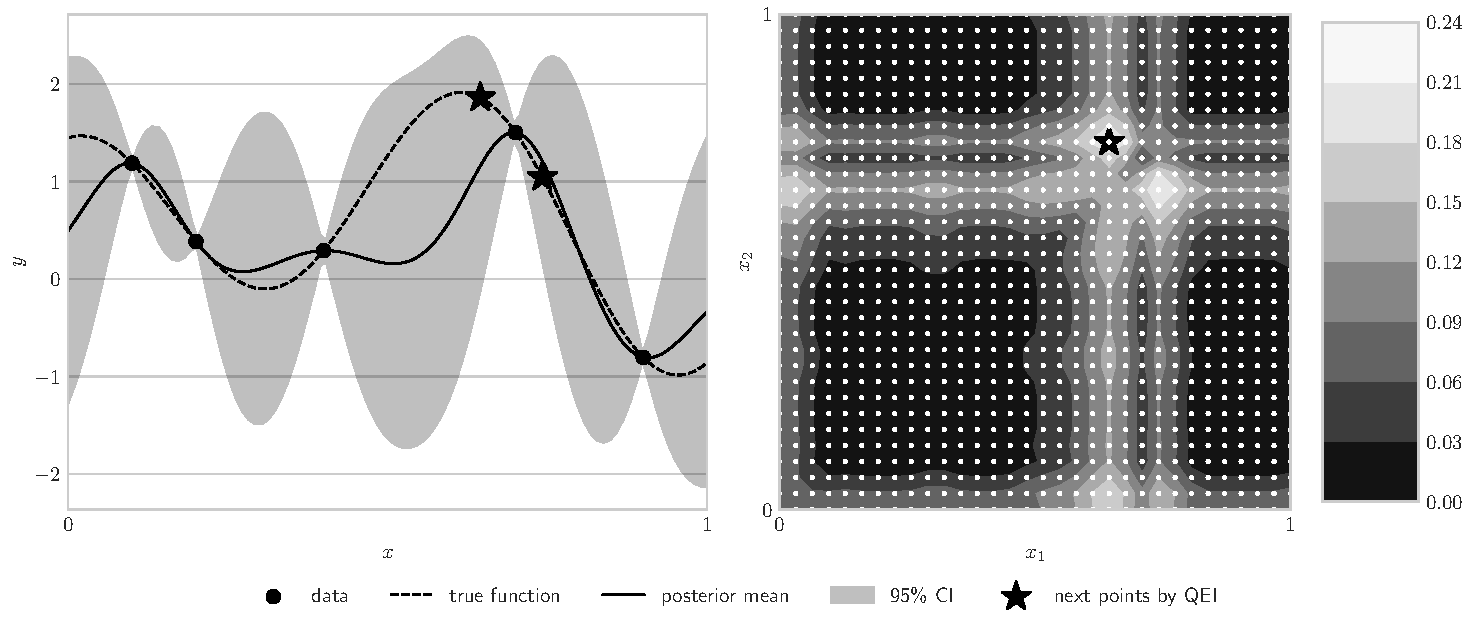
\includegraphics[width=\textwidth]{figs/gp.pdf}
    \caption{First, the true function has been sampled at the data points shown in the left panel. Next, a Gaussian Process is fit to the data points to approximate the true function, also shown in the left panel. With $q=2$, a fine grid of candidates is chosen in $[0,1]^{2}$ and the acquisition function is approximated at each of these candidates. These approximations are made into a contour plot in the right panel. The discrete argument maximum among these approximations on the fine grid is the next size $q$ batch of points by qEI. These next points for sequential optimization are visualized in both the right and left panels. }
    \label{fig:bo_qei}
\end{figure}

\subsection{Bayesian Posterior Mean}

The Bayesian framework combines prior knowledge of unknown parameters $\bS$ with observational data and a likelihood function $\rho$ to construct an informed, model-aware posterior distribution on $\bS$. Suppose we have a dataset of observations $y_1,\dots,y_{N}$ taken at IID locations $\bz_1,\dots,\bz_{N}$ respectively. Then Bayes' rule may be used to write the posterior density of $\bS$ as 
$$P\left(\bS \mid y_1,\dots,y_{N}\right) = \frac{P(y_1,\dots,y_{N} \mid \bS) P(\bS)}{P\left(y_1,\dots,y_{N}\right)} = \frac{\prod_{i=1}^{N} \rho(y_i \mid \bS) P(\bS)}{\bbE\left[\prod_{i=1}^{N} \rho(y_i \mid \bS)\right]}.$$
Here the expectation is taken with respect to the prior distribution on $\bS$ with density $P(\bS)$, and $P\left(y_1,\dots,y_{N} \mid \bS \right)$ is the likelihood density which factors into the product of likelihoods $\rho(y_i \mid \bS)$ since the observation locations are IID. 

A useful quantity of interest is the posterior mean of $\bS$. In this example, the posterior mean is our combined solution $\bs$ which may be written as the ratio of expectations via
$$\bs = \bbE\left[\bS \mid y_1,\dots,y_{N}\right] = \frac{\bbE\left[\bS \prod_{i=1}^{N} \rho(y_i \mid \bS)\right]}{\bbE\left[\prod_{i=1}^{N} \rho(y_i \mid \bS)\right]}.$$
As before, the expectations are taken with respect to the prior distribution on $\bS$. In the framework of this article $\bmu \in \bbR^{2 \times d_{\bs}}$ where for $k=1,\dots,d_{\bs}$ we have 
$$\mu_{0k} = \bbE\left[S_i \prod_{i=1}^{N} \rho(y_i \mid \bS)\right], \qquad \mu_{1k} = \bbE\left[\prod_{i=1}^{N} \rho(y_i \mid \bS)\right], \qquad \text{and} \qquad s_k = \frac{\mu_{0k}}{\mu_{1k}}.$$
While $\mu_{1k}$ is the same for all $1 \leq k \leq d_{\bs}$, we opt to keep separate denominator estimates for implementation efficiency. Defining $\bC^-$ and $\bC^+$ follow from vectorizing the quotient forms in Table \ref{table:elementary_ops_Cpm} while the dependency function $\bD: \tfset^{d_{\bs}} \to \tfset^{2 \times d_{\bs}}$ may be defined by stacking row vectors of combined flags such that
$$\bD\left(\bb^{(\bs)}\right) = \begin{pmatrix} \bb^{(\bs)} \\ \bb^{(\bs)} \end{pmatrix}.$$

For a concrete example consider Bayesian logistic regression. Here the dataset contains observations $y_i \in \{0,1\}$ at locations $\bz_i = \left(z_{i1},\dots,z_{i(d_{\bs}-1)},1\right)$ for $i=1,\dots,N$ where the last column is $1$ to accommodate an intercept term. The likelihood function is given by the sigmoid function
$$\rho(y_i = 1 \mid \bS) = \frac{\exp(\bS.\bz_i)}{1+\exp(\bS.\bz_i)}$$
so that
$$P(y_1,\dots,y_N \mid \bS) = \prod_{i=1}^N \left(\frac{\exp(\bS.\bz_i)}{1+\exp(\bS.\bz_i)}\right)^{y_i} \left(1-\frac{\exp(\bS.\bz_i)}{1+\exp(\bS.\bz_i)}\right)^{1-y_i} = \prod_{i=1}^N \frac{\exp(\bS.\bz_i)^{y_i}}{1+\exp(\bS.\bz_i)}.$$

Listing \ref{py:blr} performs Bayesian logistic regression in QMCPy
%on the Haberman's Survival Dataset retrieved from the UCI Machine Learning Repository \cite{uci_ml_repo}
. Here we use a normal prior $\bS \sim \calN(\bm,\bSigma)$ so that
$$P(\bS) = \frac{\exp\left(-(\bS-\bm)^T\bSigma^{-1}(\bs-\bm)/2\right)}{\sqrt{(2\pi)^d\lvert \det(\bSigma)\rvert }}.$$
This example uses the absolute and relative error metric \eqref{eq:h_abs_and_rel}. Notice that the number of samples required to approximate each coefficient is different. 

\lstinputlisting[caption={Bayesian Logistic Regression},style=Python,label={py:blr}]{python/blr.txt}

% \subsubsection{Haberman's Dataset Example}

% Here we perform logistic regression on the Haberman's Survival Dataset retrieved from the UCI Machine Learning Repository \cite{uci_ml_repo}. This dataset concerns a study between 1958 and 1970 at the University of Chicago's Billings Hospital that tracked the survival of patients five years after undergoing treatment for breast cancer. Predictors include the age of patient at the time of operation, operation year after 1900 e.g. 65 is 1965, and number of positive auxiliary nodes detected. The binary response variable indicates the patients survival status five years after the operation. 

% We use 2/3 of the dataset for training and the remaining 1/3 for testing. The training set has 151 positive records and 54 negative records while the testing set has 74 positive records and 27 negative records. The class imbalance reflects the fact that most patients in the study survived longer than 5 years after the operation. Since we value identifying at risk patients, we seek models with a low number of false negative predictions i.e. we desire models with high recall. Table \ref{tab:lr_models} compares a Bayesian logistic model against logistic regression models fit with an Elastic net regularization penalty
% $$\min_{\bs,c} \left[\frac{1-\lambda}{2} \lVert \bs \rVert_2^2 + \lambda \lVert \bs \rVert_1+C\sum_{i=1}^N\log(\exp(-y_i(\bx_i.\bs+c))+1)\right]$$
% where $C>0$ constant and $\lambda \in [0,1]$ controls the trade-off between $l_1$ and $l_2$ regularization. The Elastic-Net models were fit using the scikit-learn Python package with the ``saga'' optimizer \cite{scikit-learn}. The Bayesian logistic regression model was fit with $\bvarepsabs=.05$, $\bvarepsrel=.5$, error metric $h$ matching \eqref{eq:h_abs_and_rel}. Note that the Bayesian logistic regression model has the highest test recall metric.  

% \begin{table}[H]
%     \centering
%     \begin{tabular}{l|rrrr|rrr}
%         Method &\multicolumn{4}{|c|}{Coefficients} &\multicolumn{3}{c}{Test Metrics \%}\\
%         {} &       Age &  1900 Year &  Auxiliary Nodes &  Intercept &  Accuracy &  Precision &   Recall \\
%         \midrule
%         % begin insert
%         Elastic-Net $\lambda=0.0$ & -1.23e-02 &   3.44e-02 &       -1.15e-01 &   1.99e-03 &     74.3 &      76.7 &   93.2 \\
%         Elastic-Net $\lambda=0.5$ & -1.20e-02 &   3.42e-02 &       -1.15e-01 &   2.03e-03 &     74.3 &      76.7 &   93.2 \\
%         Elastic-Net $\lambda=1.0$ & -1.18e-02 &   3.39e-02 &       -1.14e-01 &   2.06e-03 &     74.3 &      76.7 &   93.2 \\
%         Bayesian                & -4.14e-03 &   1.30e-01 &       -1.57e-01 &   8.03e-03 &     74.3 &      74.0 &  100.0 \\
%         % end insert
%         \bottomrule
%     \end{tabular}
%     \caption{Comparison of Logistic regression models for the Haberman dataset.}
%     \label{tab:lr_models}
% \end{table}

\subsection{Sensitivity Indices}

Sensitivity analysis quantifies how uncertainty in a functions output may be attributed to subsets of function inputs. Functional ANOVA (analysis of variance) decomposes an objective function $\tilde{f} \in L^2(0,1)^d_{\bX}$ into the sum of orthogonal functions $(\tilde{f}_u)_{u \subseteq 1:d_{\bX}}$. Here $1:d_{\bX}=\{1,\dots,d_{\bX}\}$ denotes the set of all dimensions and $\tilde{f}_u \in L^2(0,1)^{\lvert u \rvert}$ denotes a sub-function dependent only on inputs $\bx_u = (x_j)_{j \in u}$ where $\lvert u \rvert$ is the cardinality of $u$. By construction, these sub-functions sum to the objective function so that
\begin{equation}
    \tilde{f}(\bx) = \sum_{u \subseteq 1:d_{\bX}} \tilde{f}_u(\bx_u) \label{eq:fanova}
\end{equation}
\cite[Appendix A]{mcbook}. The orthogonality of sub-functions enables the variance of $\tilde{f}$ to be decomposed into the sum of variances of sub-functions. Specifically, denoting the variance of $\tilde{f}$ by $\sigma^2$, we may write
\begin{equation*}
    \sigma^2 = \sum_{u \subseteq 1:d_{\bX}} \sigma^2_u
\end{equation*}
where $\sigma^2_u$ is the variance of sub-function $\tilde{f}_u$. The sub-variance $\sigma_u$ directly quantifies the variance of $\tilde{f}$ attributable to inputs $u \subseteq 1:d_{\bX}$.  The \emph{closed and total Sobol' indices},
\begin{equation}
    \label{eq:sobol_indices}
    \underline{\tau}_u^2 = \sum_{v \subseteq u} \sigma^2_v \quad \text{and} \quad 
    \overline{\tau}_u^2 = \sum_{v \cap u \neq \emptyset} \sigma^2_v,
\end{equation}
quantify the variance attributable to subsets of $u$ and subsets containing $u$ respectively. The \emph{sensitivity indices},
\begin{equation}
    \label{eq:sensitivity_indices_og}
    \underline{s}_u = \underline{\tau}_u^2/\sigma^2 \quad \text{and} \quad 
    \overline{s}_u = \overline{\tau}_u^2/\sigma^2,
\end{equation}
normalize the Sobol' indices to quantify the proportion of variance explained by a given subset of inputs. 

Suppose one is interested in computing the closed and total sensitivity indices of $\tilde{f}$ at $u_1,\dots,u_c \in 1:d_{\bX}$.  Then we may choose the individual solutions $\bmu \in \bbR^{6 \times c}$ and combined solutions $\bs \in \bbR^{2 \times c}$ so that for $j=1,\dots,c$
\begin{align*}
    \mu_{1j} &= \underline{\tau}_{u_j}^2 = \int_{[0,1]^{2d_{\bX}}} f(\bx)[f(\bx_{u_j},\bz_{-{u_j}})-f(\bz)]\D\bx\D\bz \\
    \mu_{2j} &= \overline{\tau}_{u_j}^2 = \frac{1}{2}\int_{[0,1]^{2d_{\bX}}} [f(\bz)-f(\bx_u,\bz_{-{u_j}})]^2\D\bx\D\bz \\
    \mu_{3j} &= \mu_{4j} = \int_{[0,1]^{d_{\bX}}} f(\bx)\D\bx, \\
    \mu_{5j} &= \mu_{6j} = \int_{[0,1]^{d_{\bX}}} f^2(\bx)\D\bx, \\
    s_{1j} &= \underline{s}_{u_j} = \frac{\underline{\tau}_{u_j}^2}{\sigma^2} = \frac{\mu_{1j}}{\mu_{5j}-\mu_{3j}^2}, \qquad \text{and} \\
    s_{2j} &= \overline{s}_{u_j} = \frac{\overline{\tau}_{u_j}^2}{\sigma^2} = \frac{\mu_{2j}}{\mu_{6j}-\mu_{4j}^2}.  
\end{align*}
Here the notation
\begin{equation}
    (\bx_{u},\bz_{-u}) = \left(\begin{aligned}x_{j}, \quad & j \in u \\ z_{j}, \quad & j \notin u \end{aligned}\right)_{j=1}^{d_{\bX}}
\end{equation}
denotes a point with inputs $u$ from $\bx$ and inputs $-u=(1:d_{\bX})\cap u^c$ from $\bz$.
For $\bmu$, the first row contains closed Sobol' indices, the second row contains total Sobol' indices, the third and fourth row contain copied first moments of $\tilde{f}$, and the forth and fifth row contain copied second moments of $\tilde{f}$. As in the previous section, we have copied various individual solutions to maintain separate estimates of the first and second moments for each combined solution. For $\bs$, the first row contains closed sensitivity indices while the second row contains total sensitivity indices. 

Then bounds from individual to combined solutions may be transformed via $\bC^-,\bC^+:\bbR^{6 \times c} \to \bbR^{2 \times c}$ defined, for $j=1,\dots,c$, by  
\begin{align*}
    C_{1j}^-(\bmu^-,\bmu^+) 
    &= \text{clip}\left(\min_{\bmu \in [\bmu^-,\bmu^+]} \frac{\mu_{1j}}{\mu_{5j}-\mu_{3j}^2}\right) \\
    &= \begin{cases} 
        \text{clip}\left(\min\left(\frac{\mu_{1j}^-}{\mu_{5j}^+-\left(\mu_{3j}^-\right)^2},\frac{\mu_{1j}^-}{\mu_{5j}^+-\left(\mu_{3j}^+\right)^2}\right)\right), & \mu_{5j}^- - \left(\mu_{3j}^\pm\right)^2 >0 \\
        0, &\text{else}
    \end{cases} \\
    C_{1j}^+(\bmu^-,\bmu^+) 
    &= \text{clip}\left(\max_{\bmu \in [\bmu^-,\bmu^+]} \frac{\mu_{1j}}{\mu_{5j}-\mu_{3j}^2}\right) \\
    &= \begin{cases} 
        \text{clip}\left(\max\left(\frac{\mu_{1j}^+}{\mu_{5j}^--\left(\mu_{3j}^-\right)^2},\frac{\mu_{1j}^+}{\mu_{5j}^--\left(\mu_{3j}^+\right)^2}\right)\right), & \mu_{5j}^- - \left(\mu_{3j}^\pm\right)^2 >0 \\
        1, &\text{else}
    \end{cases}
\end{align*}
where $\text{clip}(\cdot) = \min(1,\max(0,\cdot))$ restricts values between 0 and 1. Similarly, we may compute $C_{2j}^-$ by replacing indices 1,3,5 in $C_{1j}^-$ with indices 2,4,6 respectively and likewise for computing $C_{2j}^+$ from $C_{1j}^+$. Above, we have simplified the bounds using the facts that sensitivity indices are between 0 and 1, the variance of $\tilde{f}$ is non-negative, and Sobol' indices are non-negative. 

Moreover, the dependency function $\bD:\tfset^{2 \times c} \to \tfset^{6 \times c}$ may be defined to vertically stack combined flags three times to produce individual flags so that 
\begin{equation*}
    \bD\left(\bb^{(\bs)}\right) = \begin{pmatrix} \bb^{(\bs)} \\ \bb^{(\bs)} \\ \bb^{(\bs)} \end{pmatrix}.
\end{equation*}
In the QMCPy implementation we further generalize to allow objective functions $\tilde{\bf}: (0,1)^{d_{\bX}} \to \bbR^{\tilde{\bd}_{\bmu}}$ so that $\bd_{\bmu} = (6,c,\tilde{\bd}_{\bmu})$ and $\bd_{\bs} = (2,c,\tilde{\bd}_{\bmu})$.

Sensitivity indices present an important special case for computational complexity. Say our QMC algorithm takes $2^m$ total samples to accurately approximate closed and total sensitivity indices for $u_1,\dots,u_c \subseteq 1:d_{\bX}$. Then the computational cost is $\$(\tilde{\bf})(2+c)2^m$ since every time our sensitivity index function is evaluated at $(\bx,\bz) \in [0,1]^{2d}$ we must evaluate the users objective function at $\bx$, $\bz$, and $(\bx_{u_j},\bz_{-{u_j}})$ for $j=1,\dots,c$. Also note that when $\tilde{\bf}$ is defined to take samples in  $(0,1)^{d_{\bX}}$ to outcomes in $\bbR^{\tilde{\bd}_{\bmu}}$, sensitivity index approximation requires a wrapper taking samples in $(0,1)^{2d_{\bX}}$ to outcomes in $\bbR^{\bd_{\bmu}}$

If a user is only interested in approximating singleton sensitivity indices, $u_j = \{j\}$ for $j=1,\dots,d_{\bX}$, then it is possible to reduce the cost from $\$(\tilde{\bf})(2+d_{\bX})2^m$ to $\$(\tilde{\bf})2^{m+1}$ using order $1$ replicated designs \cite{alex2008comparison,tissot2015randomized}. Such designs have been extended to  digital sequences in \cite{replicated_designs_sobol_seq} and utilized for sensitivity index approximation in \cite{reliable_sobol_indices_approx}. In the future, we plan to optimize QMCPy to utilize replicated designs when the opportunity arises.

Recall the Ishigami function defined in \eqref{eq:ishigami}. For the Ishigami function with $a=7$, $b=0.1$ as in \cite{crestaux2007polynomial,marrel2009calculations}, Figure \ref{fig:ishigami_fu} shows exact functional ANOVA sub-functions $f_u$ for select $u \in 1:d_{\bX}$ and Figure \ref{fig:ishigami} shows approximate sensitivity indices. 

\begin{figure}[H]
    \centering
    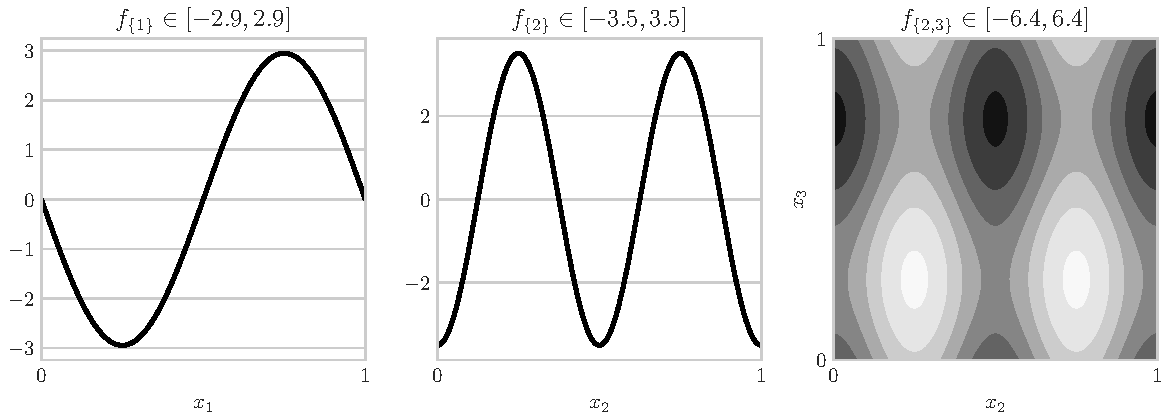
\includegraphics[width=.8\textwidth]{figs/ishigami_fu.pdf}
    \caption{Select analytic Ishigami sub-functions $f_u$ for $u \in 1:d$ from \eqref{eq:fanova}.}
    \label{fig:ishigami_fu}
\end{figure}

\begin{figure}[H]
    \centering
    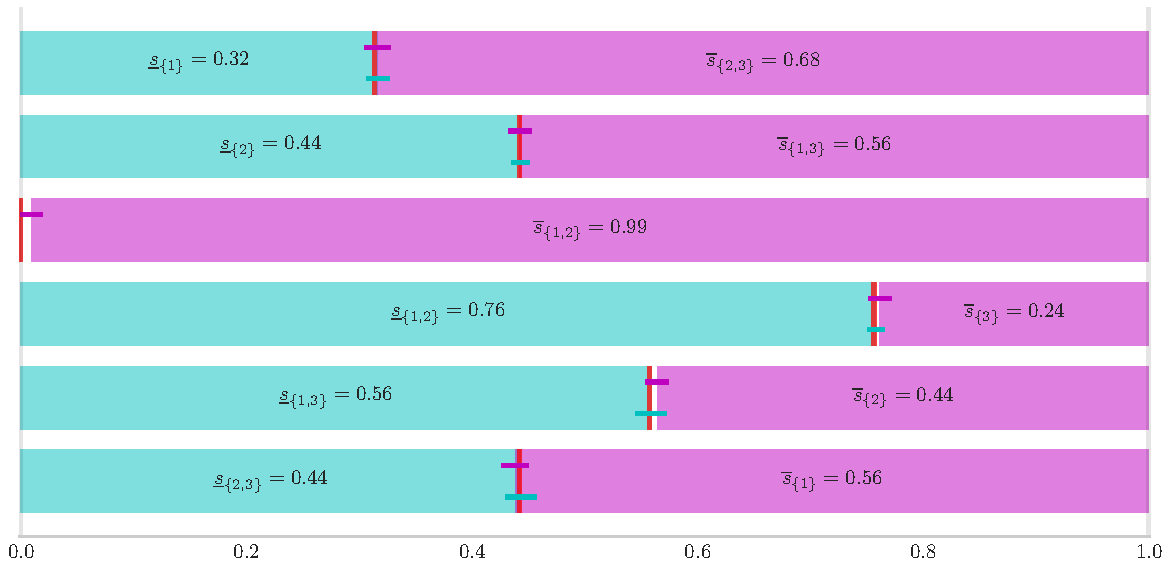
\includegraphics[width=.8\textwidth]{figs/ishigami.pdf}
    \caption{Approximate closed and total sensitivity indices for the Ishigami function illustrating the relationship $\underline{s}_u + \overline{s}_{u^c} = 1$ for $u \in 1:d$. In each row the \AGSNote{cyan} bar corresponds to a closed sensitivity index extended to the right from $0$ while the \AGSNote{magenta} bar corresponds a total sensitivity index extended to the left from $1$. The bars should meet at the \AGSNote{red} line for the  analytic solution $1-\underline{s}_u=1-\overline{s}_{u^c}$. The \AGSNote{cyan}, \AGSNote{magenta} horizontal line visualizes the combined error bounds for the closed, total sensitivity indices respectively. The \AGSNote{red} line crossing the \AGSNote{cyan} and \AGSNote{magenta} lines in each row indicates the true solution is indeed captured in the combined error bounds as desired.}
    \label{fig:ishigami}
\end{figure}

\subsubsection{Neural Network Classifier for Iris Dataset}

In this example we compute sensitivity indices of a neural network classifier for the Iris dataset retrieved from the UCI Machine Learning Repository \cite{uci_ml_repo}. This example was inspired by a similar approximation in \cite{hoyt2021efficient}. The Iris dataset consists of input features \emph{sepal length (cm)}, \emph{sepal width (cm)}, \emph{petal length (cm)}, and \emph{petal width (cm)} from which an Iris is to be classified as either the \emph{setosa}, \emph{versicolor}, or \emph{virginica} species. We begin by fitting a neural network classifier \cite{he2015delving} which takes in input features and outputs a size $3$ vector of probabilities for each species summing to $1$. Taking the argument maximum among these three probabilities gives a species prediction. On a held out portion of the dataset the neural network attains 98\% classification accuracy and may therefore be deemed a high quality surrogate for the true relation between input features and species classification. 

Our problem is to quantify, for each species, the variability in the classification probability attributed to a set of inputs. In other words, we would like to compute the sensitivity indices for each species probability. In Listing \ref{py:nn} below we compute all sensitivity indices with the help of the scikit-learn package \cite{scikit-learn} for creating a holdout dataset and training the neural network classifier. Note that $\bd_{\bmu} = (6,14,3)$ and $\bd_{\bs} = (2,14,3)$ since we have $3$ classes, $14$ sensitivity indies of interest, and we are computing both the closed and total sensitivity indices which rely on $6$ expectations per pair. Figure \ref{fig:nn_si} visualizes approximate closed sensitivity indices. 

\lstinputlisting[caption={Neural Network Sensitivity Indices},style=Python,label={py:nn}]{python/nn.txt}

\begin{figure}[H]
    \centering
    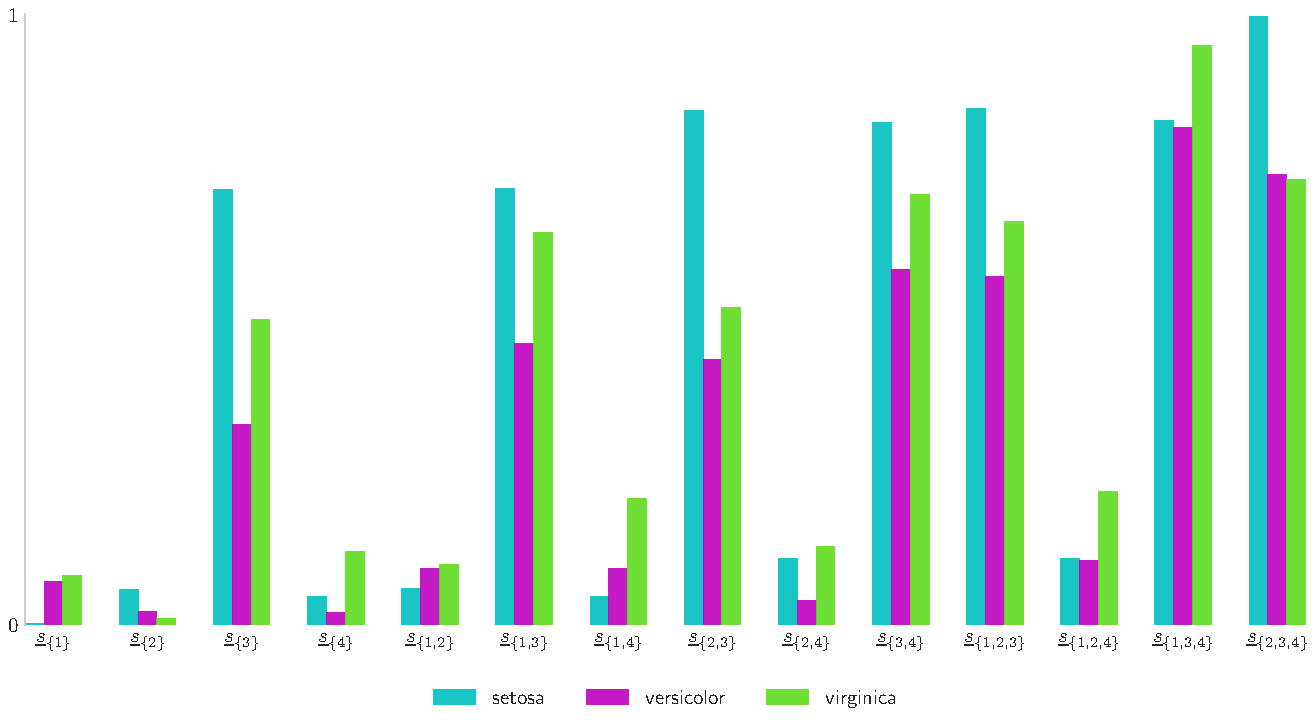
\includegraphics[width=.8\textwidth]{figs/nn_si.pdf}
    \caption{Closed sensitivity indices for neural network classification probability of each Iris species.}
    \label{fig:nn_si}
\end{figure}

\section{Conclusion}

This article has extended adaptive MC and QMC stopping criteria to support multidimensional quantities of interest formulated from multidimensional expectations. The framework is compatible with any algorithms providing probabilistic or guaranteed error bounds derived from function evaluations at IID or LD sequences. Our framework has been implemented into the open-source QMCPy package. 

\printbibliography

\section*{TODO}

\subsection*{Article}

\begin{itemize}
    \item \AGSNote{go into details about Haberman's dataset used for logistic regression example? Compare with other logistic regression techniques?} 
    \item \AGSNote{Future work section?}
    \item \AGSNote{unclear / inconsistent notation?}
\end{itemize}

\subsection*{Code}

\begin{itemize}
    \item \AGSNote{Figure \ref{fig:nn_si} xticklabels feature names instead of indices}
    \item \AGSNote{Allow custom function to take in array of functions to construct vectorized functions.}  
    \item \AGSNote{Allow QMCPy to construct a true measure from a list of 1d measures acting as independent independent marginals. Allow QMCPy to construct a true measure from an  ndarray of true measures each corresponds to one of the vector functions.} 
     \item \AGSNote{\texttt{CubBayes} algorithms allow ndarray of \texttt{abs\_tol} and \texttt{rel\_tol} and \texttt{error\_fun}}
     \item \AGSNote{New PyPI release}
\end{itemize}

\subsection*{Other}

\begin{itemize}
    \item 
\end{itemize}

\end{document}
